% LaTeX file for resume
% This file uses the resume document class (res.cls)
\documentclass[11pt]{article}
\usepackage[utf8]{inputenc}



\usepackage[usenames, dvipsnames]{xcolor}
\usepackage[colorlinks = true,urlcolor = BrickRed,pdfnewwindow=true]{hyperref}


\usepackage{datetime}
\newdateformat{yeardate}{ \THEYEAR}


\usepackage[framemethod=tikz]{mdframed}
\newmdenv[innerlinewidth=0.8pt, roundcorner=4pt,linecolor=RoyalBlue,innerleftmargin=6pt,
innerrightmargin=6pt,innertopmargin=6pt,innerbottommargin=6pt]{mybox}
\usepackage{wrapfig}

\usepackage{titlesec}
\titleformat{\section}[block]{\large}{\textbf{\thesection}}{1em}{ \bfseries}
\titleformat{\subsection}[block]{\hspace{0.6em}}{\textbf{\thesubsection}}{1em}{\bfseries}

\usepackage{etaremune}

\usepackage{fancyhdr}  % use this package to get a 2 line header
\renewcommand{\headrulewidth}{0pt} % suppress line drawn by default by fancyhdr


\pagestyle{fancy}     % set pagestyle for document
\rhead{} % put text in header (right side)

\usepackage{lastpage}
% \rhead{\textcolor{gray}{ \thepage/\pageref*{LastPage}}}

\chead{\textcolor{Gray}{}} % put text in header (right side)
\cfoot{}
\rhead{}

\rfoot{\href{https://johanmazoyer.com/}{johanmazoyer.com}}

\setlength{\parindent}{0pt}

\setlength{\headwidth}{6.5in} % taille de l'entete
\usepackage[total={6.5in,9in},left=1in,top=1in,headheight=110pt]{geometry} %%%%% 8.5in x 11in




\begin{document}
\lhead[]{}
\lfoot{\textcolor{Gray}{CV last update: \yeardate\today}}
% \textcolor{white}{.}
% \vspace{-1.cm}

\begin{huge}
\noindent\textbf{Johan MAZOYER}
\end{huge}\\

%\vspace{-0.3cm}
%\textit{French citizen, born on December $14^{th}$ 1986, Paris, France.}

\textbf{Research Interests: Optical Instrumentation, Direct Imaging \& Coronagraphy,
Observation \& Characterization of Extrasolar Systems, Debris Disks}\\


%%%%%%%%%%%%%%%%%%%%%%%%%%%%%%%%%%%%%%%%%%%%%%%%%%%%%%%%%%%%%%%%%%%%%%%%%%%%%%%%%%%%%%%%%%%%%%%%%%%%%%%%%%%%%%%%%%%%%%%%
%%%%%% SECTION RESEARCH EXPERIENCE
%%%%%%%%%%%%%%%%%%%%%%%%%%%%%%%%%%%%%%%%%%%%%%%%%%%%%%%%%%%%%%%%%%%%%%%%%%%%%%%%%%%%%%%%%%%%%%%%%%%%%%%%%%%%%%%%%%%%%%%%
\vspace{-1cm}
\textcolor{RoyalBlue}{\section{\large RESEARCH POSITIONS}
\vspace{-0.35cm}\hrule}
\vspace{0.4cm}

\textbf{CNRS Scientist} --
\href{http://www.obspm.fr/?lang=en}{\textbf{LESIA/Paris Observatory - PSL}} (France)
\hfill     	 { \bf Since 2020}\\


\textbf{Carl Sagan Fellow} --
\href{https://www.jpl.nasa.gov/}{\textbf{NASA Jet Propulsion Laboratory}} (Pasadena, CA)
\hfill      { \bf 2018 - 2019}\\


\textbf{Postdoc} --
\href{http://physics-astronomy.jhu.edu/}{\textbf{Johns Hopkins University}} (Baltimore, MD)
\hfill   	 { \bf 2016 - 2018}\\


\textbf{Postdoc} --
{\href{http://www.stsci.edu}{\textbf{Space Telescope Science Institute}}} (Baltimore, MD)
\hfill        { \bf 2014 - 2016}\\

\textbf{Graduate Student} --
\href{http://www.obspm.fr/?lang=en}{\textbf{LESIA/Paris Observatory - PSL}} (France)
\hfill        { \bf 2011 - 2014}\\


% \vspace{-0.1cm}
% {\small \textbf{Visiting Research Student} -- \href{http://www.lanl.gov/}{\textbf{Los Alamos National Laboratory} } \hfill    	Los Alamos, NM\\
% MSL/ChemCam Collaboration (Roger Wiens) \hfill  		 \textbf{Summer 2011}\\

% \vspace{-0.1cm}
% \textbf{Visiting Research Student} -- \href{http://www.irap.omp.eu/en}{\textbf{IRAP}} \hfill    	Toulouse, Fr\\
% MSL/ChemCam Collaboration (Olivier Gasnault \& Sylvestre Maurice) \hfill		  \textbf{Spring 2011}}\\

%\vspace{-0.35cm}
%{\small \textbf{CNES} (French space agency) \hfill    	Toulouse, France\\
%\textit{Master student} ; Pleiades satellites \hfill  		 {\bf March -- July 2010}}\\
%
%\vspace{-0.35cm}
%{\small\textbf{Le Relais} (French NGO) \hfill    		  Koudougou, Burkina Faso\\
%Humanitarian work\hfill  		  {\bf July -- Sept. 2009}}	\\

%%%%%%%%%%%%%%%%%%%%%%%%%%%%%%%%%%%%%%%%%%%%%%%%%%%%%%%%%%%%%%%%%%%%%%%%%%%%%%%%%%%%%%%%%%%%%%%%%%%%%%%%%%%%%%%%%%%%%%%%
%%%%%% SECTION EDUCATION
%%%%%%%%%%%%%%%%%%%%%%%%%%%%%%%%%%%%%%%%%%%%%%%%%%%%%%%%%%%%%%%%%%%%%%%%%%%%%%%%%%%%%%%%%%%%%%%%%%%%%%%%%%%%%%%%%%%%%%%%

\vspace{-0.25cm}
\textcolor{RoyalBlue}{\section{\large EDUCATION}
\vspace{-0.35cm}\hrule}
\vspace{0.4cm}

\textbf{HDR} --
\href{http://www.obspm.fr}{\textbf{Paris Observatory - PSL}} (France)
\hfill  { \bf 03/2024}\\


\textbf{PhD} -- Astronomy \& Astrophysics --
\href{https://www.univ-paris-diderot.fr/}{\textbf{Universit\'e Paris Diderot}} (France)
\hfill  { \bf 09/2014}\\
{\small
\null \hspace{0.6cm}
{\it Thesis}: High-Contrast Imaging Of Exoplanets And Circumstellar Disks (P. Baudoz \& G. Rousset)}\\

% \vspace{-0.1cm}
\textbf{Master} -- Astrophysics --
\href{http://ezomp2.omp.obs-mip.fr/asep/index.php/eng}{\textbf{Université Paul Sabatier}} (Toulouse, France)
\hfill  { \bf 09/2011} \\
{\small
\null \hspace{0.6cm}
{\it Thesis}: Influence of Mars atmosphere on ChemCam detection limits (O. Gasnault \& R. Wiens)}\\

% \vspace{-0.1cm}
\textbf{Master} -- Space Engineering -- \href{https://www.isae-supaero.fr/en/}{\textbf{\textbf{ISAE Supaero}}} (Toulouse, France) \hfill  { \bf 09/2011} \\

% \vspace{-0.1cm}
\textbf{Bachelor} -- Computer Science -- \href{http://www.polytechnique.edu/en/}{\textbf{\textbf{Ecole polytechnique}}} (Paris, France) \hfill    { \bf 09/2010}\\





%%%%%%%%%%%%%%%%%%%%%%%%%%%%%%%%%%%%%%%%%%%%%%%%%%%%%%%%%%%%%%%%%%%%%%%%%%%%%%%%%%%%%%%%%%%%%%%%%%%%%%%%%%%%%%%%%%%%%%%%
%%%%%% SECTION AWARDS
%%%%%%%%%%%%%%%%%%%%%%%%%%%%%%%%%%%%%%%%%%%%%%%%%%%%%%%%%%%%%%%%%%%%%%%%%%%%%%%%%%%%%%%%%%%%%%%%%%%%%%%%%%%%%%%%%%%%%%%%

\vspace{-0.25cm}
\textcolor{RoyalBlue}{\section{\large GRANTS \& AWARDS}
\vspace{-0.35cm}\hrule}
\vspace{0.4cm}
\textbf{Franco-Chilean Collaboration Program} \href{https://www.univ-paris13.fr/ecos-sud/}{EcosSud} with {\it Universidad de Chile} -- 3 yrs \hfill   \textbf{2020}\\ %- \$300K/3 yrs

\vspace{-0.2cm}
\textbf{NASA Group Award}: LBTI Hosts Survey Science Team \hfill   \textbf{2020}\\ 

\vspace{-0.2cm}
\textbf{Carl Sagan Fellowship} (\href{http://www.stsci.edu/stsci-research/fellowships/nasa-hubble-fellowship-program}{NASA Hubble Fellowship Program}) -- 3 yrs \hfill   \textbf{2018}\\ %- \$300K/3 yrs

\vspace{-0.2cm}
Cover of \textbf{Astronomy \& Astrophysics} Journal (\href{https://www.aanda.org/articles/aa/abs/2014/04/contents/contents.html}{Volume 564}) \hfill  \textbf{2014}\\

% \vspace{-0.2cm}
% \textbf{Outstanding Presentation Award} (CNES fellow symposium JC$^2$) \hfill   \textbf{2013}\\

\vspace{-0.2cm}
\textbf{CNES Doctoral Research Fellowship} (\href{https://cnes.fr/en/web/CNES-en/7430-research-grants.php}{French space agency}) -- 3 yrs  \hfill   \textbf{2011}\\ %- \$66K/3 yrs

\vspace{-0.2cm}
\textbf{Ecole Polytechnique Scholarship} -- 4 yrs   \hfill   \textbf{2007}\\

%%%%%%%%%%%%%%%%%%%%%%%%%%%%%%%%%%%%%%%%%%%%%%%%%%%%%%%%%%%%%%%%%%%%%%%%%%%%%%%%%%%%%%%%%%%%%%%%%%%%%%%%%%%%%%%%%%%%%%%%
%%%%%% SECTION VULGARISATION
%%%%%%%%%%%%%%%%%%%%%%%%%%%%%%%%%%%%%%%%%%%%%%%%%%%%%%%%%%%%%%%%%%%%%%%%%%%%%%%%%%%%%%%%%%%%%%%%%%%%%%%%%%%%%%%%%%%%%%%%

\newpage
\lfoot{}
\textcolor{White}{.}
%\lhead{\textcolor{Gray}{J. MAZOYER}}
\vspace{-1.5cm}
\textcolor{RoyalBlue}{\section{\large OUTREACH}
\vspace{-0.35cm}\hrule}
\vspace{0.5cm}
\begin{wrapfigure}{l}{0.17\textwidth}
\vspace{-0.95cm}
\begin{mybox}
    
\includegraphics[width=1.\textwidth]{figures_CV/PodcastScience.png}
 \end{mybox}
\vspace{-1.1cm}
\end{wrapfigure}
\textbf{Podcast Science}: I am running \href{http://www.podcastscience.fm}
{\textbf{PodcastScience.fm}}, a \textbf{general science program}, airing every
Wednesdays, in french. This podcast is listened by 10'000 to 20'000
listeners. Podcast Science received the Golden blog award for
best scientific blog in 2012.

\vspace{0.2cm}

\textbf{Public talks}: CERN \& Palais de la découverte (Paris)\\

\vspace{-0.35cm}
\textcolor{RoyalBlue}{\section{\large PROFESSIONAL ACTIVITIES \& SERVICE}
\vspace{-0.35cm}\hrule}
\vspace{0.4cm}

% \parbox{0.58\linewidth}{
\textbf{Conference, Workshop and Seminar Organizer:}
\vspace{0.3cm}
\begin{itemize} \itemsep -2pt
 \item \small Seminar \textbf{``Haute Résolution Angulaire pour l'Astrophysique" (HRAA)} at LESIA (2020-)
 \item \small Organizer and SOC: \textbf{National Capital Area Disks} workshop (Baltimore, MD, Oct. 2018) - \href{https://sites.google.com/view/ncad7-at-jhu/ncad7}{\underline{\textbf{website}}}
 \item \small Organizer and SOC: \textbf{Optimal Optical Coronagraphs} workshop (Leiden, NL, Sep. 2017) - \href{https://www.lorentzcenter.nl/lc/web/2017/924/info.php3?wsid=924&venue=Snellius}{\underline{\textbf{website}}}
 \item \small Seminar \textbf{``Exoplanet Star and Planet Formation" (ESPF)} at STScI (2016-2018)
 \item \small SOC: \textbf{High Contrast Imaging from Space} (Baltimore, MD, Nov. 2016) - \href{http://www.cvent.com/events/high-contrast-imaging-in-space-workshop/event-summary-eb3bb6bd54a342c5a15678daa49be683.aspx}{\underline{\textbf{website}}}
 \item \small LOC: Workshop \textbf{très haute dynamique} (Paris, 2012)
\end{itemize}
\vspace{0.1cm}
\textbf{Other Services:}
\begin{itemize} \itemsep -2pt
    \item \small \textbf{Hubble \textit{Telescope Allocation Committee}} \hfill 2024
    \item \small Head of high-contrast imaging team at LESIA \hfill 2023 - 
    \item \small Science Commity of CNRS/INSU's exoplanets group \textbf{(CET exoplanètes)}  \hfill 2023 - 
    \item \small \textbf{Roman:} Deputy CNES representative in Community Participation Program (CPP) Team  \hfill 2023 - 
    \item \small \textbf{SPHERE+:} Responsible of the Focal Plane Wavefront Sensor working group \hfill 2022 - 
    \item \small Science Commity of CNRS/INSU's High Angular Resolution Group \textbf{(CS-ASHRA)} \hfill 2021 - 
    \item \small \textbf{Habitable Exoplanet Observatory (HabEx)}: Contributing Scientist \hfill 2019
    \item \small \textbf{Large UV Optical Infrared Surveyor (LUVOIR)}: Contributing Scientist \hfill 2019
    \item \small IAU Junior member \hfill 2019 - 
    % \item \small NASA Exoplanet Exploration Program Analysis Group (ExoPAG) member of the \textbf{Study Analysis Groups (SAGs) \#19} (Theory and Rigorous Contrast Metrics).
    \item \small \textbf{Referee} for publications in the \textit{AJ}, \textit{A}\&\textit{A}, \textit{MNRAS}, \textit{PASP} and \textit{JATIS}.
\end{itemize}


% \begin{mybox}
%     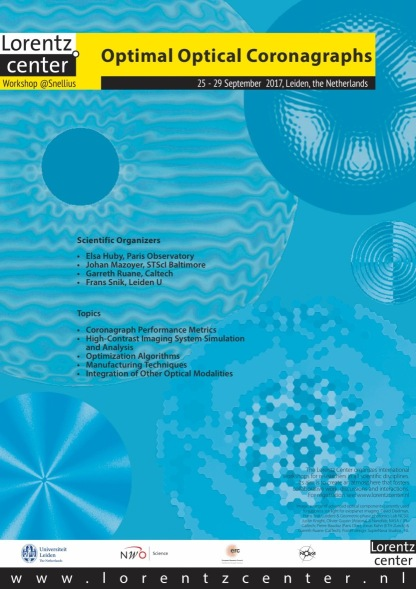
\includegraphics[width=1.\textwidth]{figures_CV/ooc_poster2_sm.jpg}
%  \end{mybox}
% }



% \begin{itemize}
%     % \item \small NASA Exoplanet Exploration Program Analysis Group (ExoPAG) member of the \textbf{Study Analysis Groups (SAGs) \#19} (Theory and Rigorous Contrast Metrics) since 2016 (see Jensen-Clem et al. 2018).
%     % \item \small Development of the \textbf{Paris THD optical testbed website} in August 2014.
%     \item \small \textbf{Referee} for publications in the \textit{AJ}, \textit{A}\&\textit{A}, \textit{MNRAS}, \textit{PASP} and \textit{JATIS}.
% \end{itemize}

%\vspace{-1.cm}
%\textcolor{RoyalBlue}{\section{\large MAIN OBSERVATION CAMPAIGNS}
%\vspace{-0.35cm}\hrule}
%\vspace{0.22cm}
%
%\textbf{Palomar Observatory (200 inch telescope)}
%
%\begin{itemize} \itemsep -1pt % reduce space between items
%	    \item \small Mai 2015, 3 nights -- First on-sky test of the Self-Coherent Camera
%\end{itemize}
%
%\textbf{Gemini South/GPI}
%\vspace{-0.2cm}
%\begin{itemize} \itemsep -1pt % reduce space between items
%	    \item \small December 2015, 1 week -- Remote observing and data reduction
%		\item \small March 2016, 1 week --  Remote observing and data reduction
% 	\item \small October 2016, 1 week --  On-site observing and data reduction\\
%Since the end of 2016, all south Gemini observations are carried out remotely.
% 	\item \small December 2016, 4 nights --  Assistance and data reduction
% 	\item \small December 2017, 3 nights --  Assistance and data reduction
% 	\item \small January 2018, 4 nights --  Remote observing and data reduction
%\end{itemize}

%%%%%%%%%%%%%%%%%%%%%%%%%%%%%%%%%%%%%%%%%%%%%%%%%%%%%%%%%%%%%%%%%%%%%%%%%%%%%%%%%%%%%%%%%%%%%%%%%%%%%%%%%%%%%%%%%%%%%%%%
%%%%%% Demandes de temps
%%%%%%%%%%%%%%%%%%%%%%%%%%%%%%%%%%%%%%%%%%%%%%%%%%%%%%%%%%%%%%%%%%%%%%%%%%%%%%%%%%%%%%%%%%%%%%%%%%%%%%%%%%%%%%%%%%%%%%%%

%\vspace{-0.8cm}
%\textcolor{RoyalBlue}{\section{\large OBSERVATION PROPOSALS}
%\vspace{-0.35cm}\hrule}
%\vspace{0.4cm}
%
%\textbf{GEMINI/GPI}\\
%\vspace{-0.4cm}
%\begin{itemize} \itemsep -3pt % reduce space between items
%    \item \small GS-2015B-LP-6 ``Characterizing Dusty Debris in Exoplanetary Systems'' (PI: Christine Chen)\\
%\end{itemize}
%
%\vspace{-0.4cm}
%\textbf{VLT/SPHERE}
%\vspace{-0.2cm}
%\begin{itemize} \itemsep -3pt % reduce space between items
%    \item \small P 098.C-0686 ``Resolving multiple belts and sub-structures in inner regions of highly inclined debris disk" (PI: Anthony Boccaletti)
%    \item \small P 096.C-0640 ``Exploring the inner cavities of two very inclined debris disks'' (PI: Anthony Boccaletti)
%    \item \small P 095.C-0381 ``Investigating the inner part of a transitional disk"'' (PI: Anthony Boccaletti)
%\end{itemize}
%
%\textbf{JWST / MIRI, NIRCam, NIRSPEC \& NIRISS}
%\vspace{-0.2cm}
%\begin{itemize} \itemsep -3pt % reduce space between items
%    \item \small Programme Early realease Science (ERS) ``High Contrast Imaging of Exoplanets and Exoplanetary Systems with JWST" (PI : Sasha Hinkley)
%\end{itemize}

%%%%%%%%%%%%%%%%%%%%%%%%%%%%%%%%%%%%%%%%%%%%%%%%%%%%%%%%%%%%%%%%%%%%%%%%%%%%%%%%%%%%%%%%%%%%%%%%%%%%%%%%%%%%%%%%%%%%%%%%
%%%%%% SECTION RESPONSABILITE
%%%%%%%%%%%%%%%%%%%%%%%%%%%%%%%%%%%%%%%%%%%%%%%%%%%%%%%%%%%%%%%%%%%%%%%%%%%%%%%%%%%%%%%%%%%%%%%%%%%%%%%%%%%%%%%%%%%%%%%%

% \newpage
\vspace{-0.8cm}
\textcolor{RoyalBlue}{\section{\large MENTORING}
\vspace{-0.35cm}\hrule}
\vspace{0.4cm}
{\small
\textbf{Vito Squicciarini} (Postdoc, LESIA): co-advisor with A.-M. Lagrange \hfill \textbf{Since 2022}\\
\textbf{Yann Gutierrez} (PhD, LESIA): co-advidor with L. Mugnier, ONERA \hfill \textbf{Since 2022}\\
\textbf{Iva Laginja} (Postdoc, LESIA): CNES post-doctoral Fellow \hfill \textbf{Since 2022}\\
\textbf{Sophia Stasevic} (PhD, LESIA) co-advisor with A.-M. Lagrange and J. Milli \hfill \textbf{Since 2021}\\
\textbf{Justin Hom} (PhD, ASU) co-advisor with J. Patience \hfill \textbf{2019 - 2023}\\
\textbf{Kevin Fogarty} (PhD, JHU) co-advisor with L. Pueyo. Now Research Scientist at AMES \hfill \textbf{2017-2019}\\
}
% \newpage
\vspace{-0.cm}
\textcolor{RoyalBlue}{\section{\large TEACHING}
\vspace{-0.35cm}\hrule}
\vspace{0.4cm}
% \vspace{-0.2cm}
Observatoire de Paris Master Class: 
\begin{itemize} \itemsep -2pt
    \item Instrumentation for Astronomy 
    \item Detection of Exoplanets (collab. Anne-Marie Lagrange)
\end{itemize}

% \textbf{Teaching assistant}  \hfill  Paris 7 \&  Paris 5 Universities  \hfill \textbf{2011 - 2014}\\


% \textbf{La Main à la Pâte:} \hfill \textbf{2007 - 2008}\\
%  {\small I taught science during 8 months (30h/week) in primary schools in underprivileged 
%     neighborhoods (Perpignan, Fr) for the 
%     \href{https://www.fondation-lamap.org/en/international}{\textbf{La Main à la pâte}} organization.} 





%\vspace{-0.5cm}
%\textcolor{RoyalBlue}{\section{\large  SPORT}
%\vspace{-0.35cm}\hrule}
%\vspace{0.4cm}
%\textbf{Fencing} (15 years of practice) \& \textbf{Running} (trails, half-marathons, marathon)\\

% \newpage

% \textcolor{White}{.}
% \vspace{-1.cm}
% \begin{center}
% \begin{Large}
% \textbf{PUBLICATIONS}\\
% \end{Large}
% \setcounter{section}{0}
% \end{center}


% \vspace{-0.8cm}
% \textcolor{RoyalBlue}{\section{MAJOR REFEREED PUBLICATIONS}
% \vspace{-0.25cm}\hrule}
% \vspace{0.6cm}
% \begin{etaremune}\itemsep 0pt
% \item {\bf Mazoyer, J.} ; Pueyo, L. ; N'Diaye, M. et al. ({\bf2018}), {\it Active Correction of Aperture Discontinuities-Optimized Stroke Minimization. II. Optimization for Future Missions}, The Astronomical Journal, 155, 8, \href{https://ui.adsabs.harvard.edu/abs/2018AJ....155....8M/abstract}{ADS Link}, 7 citations

% \item {\bf Mazoyer, J.} ; Pueyo, L. ; N'Diaye, M. et al. ({\bf2018}), {\it Active Correction of Aperture Discontinuities-Optimized Stroke Minimization. I. A New Adaptive Interaction Matrix Algorithm}, The Astronomical Journal, 155, 7, \href{https://ui.adsabs.harvard.edu/abs/2018AJ....155....7M/abstract}{ADS Link}, 6 citations

% \item Fogarty, K. ; Pueyo, L. ; {\bf Mazoyer, J.} et al. ({\bf2017}), {\it Polynomial Apodizers for Centrally Obscured Vortex Coronagraphs}, The Astronomical Journal, 154, 240, \href{https://ui.adsabs.harvard.edu/abs/2017AJ....154..240F/abstract}{ADS Link}, 6 citations

% \item {\bf Mazoyer, J.} ; Pueyo, L. ; Norman, C. et al. ({\bf2016}), {\it Active compensation of aperture discontinuities for WFIRST-AFTA: analytical and numerical comparison of propagation methods and preliminary results with a WFIRST-AFTA-like pupil}, Journal of Astronomical Telescopes, Instruments, and Systems, 2, 011008, \href{https://ui.adsabs.harvard.edu/abs/2016JATIS...2a1008M/abstract}{ADS Link}, 7 citations

% \item {\bf Mazoyer, J.} ; Boccaletti, A. ; Choquet, É. et al. ({\bf2016}), {\it A Symmetric Inner Cavity in the HD 141569A Circumstellar Disk}, The Astrophysical Journal, 818, 150, \href{https://ui.adsabs.harvard.edu/abs/2016ApJ...818..150M/abstract}{ADS Link}, 9 citations

% \item {\bf Mazoyer, J.} ; Boccaletti, A. ; Augereau, J. -C. et al. ({\bf2014}), {\it Is the HD 15115 inner disk really asymmetrical?}, Astronomy and Astrophysics, 569, A29, \href{https://ui.adsabs.harvard.edu/abs/2014A&A...569A..29M/abstract}{ADS Link}, 28 citations

% \item {\bf Mazoyer, J.} ({\bf2014}), {\it High-Contrast Direct Imaging Of Exoplanets And Circumstellar Disks: From The Self-Coherent Camera To Nici Data Analysis}, Ph.D. Thesis, \href{https://ui.adsabs.harvard.edu/abs/2014PhDT.......497M/abstract}{ADS Link}, 2 citations

% \item {\bf Mazoyer, J.} ; Baudoz, P. ; Galicher, R. et al. ({\bf2014}), {\it High-contrast imaging in polychromatic light with the self-coherent camera}, Astronomy and Astrophysics, 564, L1, \href{https://ui.adsabs.harvard.edu/abs/2014A&A...564L...1M/abstract}{ADS Link}, 23 citations

% \item {\bf Mazoyer, J.} ; Baudoz, P. ; Galicher, R. et al. ({\bf2013}), {\it Estimation and correction of wavefront aberrations using the self-coherent camera: laboratory results}, Astronomy and Astrophysics, 557, A9, \href{https://ui.adsabs.harvard.edu/abs/2013A&A...557A...9M/abstract}{ADS Link}, 23 citations

% \end{etaremune}


% \vspace{-0.8cm}
% \textcolor{RoyalBlue}{\section{OTHER REFEREED PUBLICATIONS}
% \vspace{-0.25cm}\hrule}
% \vspace{0.6cm}
% \begin{etaremune}\itemsep 0pt
% \item Bhowmik, T. et al. ({\bf2019}), {\it Spatially resolved spectroscopy of the debris disk HD 32297. Further evidence of small dust grains}, Astronomy and Astrophysics, 630, A85, \href{https://ui.adsabs.harvard.edu/abs/2019A&A...630A..85B/abstract}{ADS Link}, 1 citation

% \item Ren, B. et al. ({\bf2019}), {\it An Exo-Kuiper Belt with an Extended Halo around HD 191089 in Scattered Light}, The Astrophysical Journal, 882, 64, \href{https://ui.adsabs.harvard.edu/abs/2019ApJ...882...64R/abstract}{ADS Link}

% \item Stark, C. C. et al. ({\bf2019}), {\it ExoEarth yield landscape for future direct imaging space telescopes}, Journal of Astronomical Telescopes, Instruments, and Systems, 5, 024009, \href{https://ui.adsabs.harvard.edu/abs/2019JATIS...5b4009S/abstract}{ADS Link}

% \item Engler, N. et al. ({\bf2019}), {\it Investigating the presence of two belts in the HD 15115 system}, Astronomy and Astrophysics, 622, A192, \href{https://ui.adsabs.harvard.edu/abs/2019A&A...622A.192E/abstract}{ADS Link}, 5 citations

% \item Esposito, T. M. et al. ({\bf2018}), {\it Direct Imaging of the HD 35841 Debris Disk: A Polarized Dust Ring from Gemini Planet Imager and an Outer Halo from HST/STIS}, The Astronomical Journal, 156, 47, \href{https://ui.adsabs.harvard.edu/abs/2018AJ....156...47E/abstract}{ADS Link}, 2 citations

% \item Leboulleux, L. et al. ({\bf2018}), {\it Pair-based Analytical model for Segmented Telescopes Imaging from Space for sensitivity analysis}, Journal of Astronomical Telescopes, Instruments, and Systems, 4, 035002, \href{https://ui.adsabs.harvard.edu/abs/2018JATIS...4c5002L/abstract}{ADS Link}, 2 citations

% \item Poteet, C. A. et al. ({\bf2018}), {\it Space-based Coronagraphic Imaging Polarimetry of the TW Hydrae Disk: Shedding New Light on Self-shadowing Effects}, The Astrophysical Journal, 860, 115, \href{https://ui.adsabs.harvard.edu/abs/2018ApJ...860..115P/abstract}{ADS Link}, 3 citations

% \item Jensen-Clem, R. et al. ({\bf2018}), {\it A New Standard for Assessing the Performance of High Contrast Imaging Systems}, The Astronomical Journal, 155, 19, \href{https://ui.adsabs.harvard.edu/abs/2018AJ....155...19J/abstract}{ADS Link}, 12 citations

% \item Fogarty, K. et al. ({\bf2017}), {\it Polynomial Apodizers for Centrally Obscured Vortex Coronagraphs}, The Astronomical Journal, 154, 240, \href{https://ui.adsabs.harvard.edu/abs/2017AJ....154..240F/abstract}{ADS Link}, 6 citations

% \item Perrot, C. et al. ({\bf2016}), {\it Discovery of concentric broken rings at sub-arcsec separations in the HD 141569A gas-rich, debris disk with VLT/SPHERE}, Astronomy and Astrophysics, 590, L7, \href{https://ui.adsabs.harvard.edu/abs/2016A&A...590L...7P/abstract}{ADS Link}, 18 citations

% \item Delorme, J. R. et al. ({\bf2016}), {\it Focal plane wavefront sensor achromatization: The multireference self-coherent camera}, Astronomy and Astrophysics, 588, A136, \href{https://ui.adsabs.harvard.edu/abs/2016A&A...588A.136D/abstract}{ADS Link}, 9 citations

% \item Choquet, É. et al. ({\bf2016}), {\it First Images of Debris Disks around TWA 7, TWA 25, HD 35650, and HD 377}, The Astrophysical Journal, 817, L2, \href{https://ui.adsabs.harvard.edu/abs/2016ApJ...817L...2C/abstract}{ADS Link}, 39 citations

% \item Debes, J. H. et al. ({\bf2016}), {\it Wide-Field Infrared Survey Telescope-Astrophysics Focused Telescope Assets coronagraphic operations: lessons learned from the Hubble Space Telescope and the James Webb Space Telescope}, Journal of Astronomical Telescopes, Instruments, and Systems, 2, 011010, \href{https://ui.adsabs.harvard.edu/abs/2016JATIS...2a1010D/abstract}{ADS Link}, 9 citations

% \item Wiens, R. C. et al. ({\bf2013}), {\it Pre-flight calibration and initial data processing for the ChemCam laser-induced breakdown spectroscopy instrument on the Mars Science Laboratory rover}, Spectrochimica Acta, 82, 1, \href{https://ui.adsabs.harvard.edu/abs/2013AcSpe..82....1W/abstract}{ADS Link}, 117 citations

% \item Cousin, A. et al. ({\bf2011}), {\it Laser induced breakdown spectroscopy library for the Martian environment}, Spectrochimica Acta, 66, 805, \href{https://ui.adsabs.harvard.edu/abs/2011AcSpe..66..805C/abstract}{ADS Link}, 39 citations

% \end{etaremune}


% \vspace{-0.8cm}
% \textcolor{RoyalBlue}{\section{MAJOR CONFERENCE PROCEEDINGS}
% \vspace{-0.25cm}\hrule}
% \vspace{0.6cm}
% \begin{etaremune}\itemsep 0pt
% \item Fogarty, K. ; {\bf Mazoyer, J.} ; St. Laurent, K. et al. ({\bf2018}), {\it Optimal deformable mirror and pupil apodization combinations for apodized pupil Lyot coronagraphs with obstructed pupils}, Space Telescopes and Instrumentation 2018: Optical, Infrared, and Millimeter Wave, 10698, 106981J, \href{https://ui.adsabs.harvard.edu/abs/2018SPIE10698E..1JF/abstract}{ADS Link}

% \item Ruane, G. ; Riggs, A. ; {\bf Mazoyer, J.} et al. ({\bf2018}), {\it Review of high-contrast imaging systems for current and future ground- and space-based telescopes I: coronagraph design methods and optical performance metrics}, Space Telescopes and Instrumentation 2018: Optical, Infrared, and Millimeter Wave, 10698, 106982S, \href{https://ui.adsabs.harvard.edu/abs/2018SPIE10698E..2SR/abstract}{ADS Link}

% \item {\bf Mazoyer, J.} ; Pueyo, L. ; N'Diaye, M. et al. ({\bf2017}), {\it Capabilities of ACAD-OSM, an active method for the correction of aperture discontinuities}, Society of Photo-Optical Instrumentation Engineers (SPIE) Conference Series, 10400, 104000G, \href{https://ui.adsabs.harvard.edu/abs/2017SPIE10400...0GM/abstract}{ADS Link}, 2 citations

% \item {\bf Mazoyer, J.} ; Pueyo, L. ({\bf2017}), {\it Fundamental limits to high-contrast wavefront control}, Society of Photo-Optical Instrumentation Engineers (SPIE) Conference Series, 10400, 1040014, \href{https://ui.adsabs.harvard.edu/abs/2017SPIE10400E..14M/abstract}{ADS Link}, 1 citation

% \item Leboulleux, L. ; N'Diaye, M. ; {\bf Mazoyer, J.} et al. ({\bf2017}), {\it Comparison of wavefront control algorithms and first results on the high-contrast imager for complex aperture telescopes (hicat) testbed}, Society of Photo-Optical Instrumentation Engineers (SPIE) Conference Series, 10562, 105622Z, \href{https://ui.adsabs.harvard.edu/abs/2017SPIE10562E..2ZL/abstract}{ADS Link}

% \item Fogarty, K. ; Pueyo, L. ; {\bf Mazoyer, J.} et al. ({\bf2017}), {\it Tip/tilt optimizations for polynomial apodized vortex coronagraphs on obscured telescope pupils}, Society of Photo-Optical Instrumentation Engineers (SPIE) Conference Series, 10400, 104000T, \href{https://ui.adsabs.harvard.edu/abs/2017SPIE10400E..0TF/abstract}{ADS Link}, 2 citations

% \item {\bf Mazoyer, J.} ; Pueyo, L. ; N'Diaye, M. et al. ({\bf2016}), {\it Correcting for the effects of pupil discontinuities with the ACAD method}, Space Telescopes and Instrumentation 2016: Optical, Infrared, and Millimeter Wave, 9904, 99044T, \href{https://ui.adsabs.harvard.edu/abs/2016SPIE.9904E..4TM/abstract}{ADS Link}

% \item {\bf Mazoyer, J.} ; Pueyo, L. ; Norman, C. et al. ({\bf2015}), {\it Active correction of aperture discontinuities (ACAD) for space telescope pupils: a parametic analysis}, Techniques and Instrumentation for Detection of Exoplanets VII, 9605, 96050M, \href{https://ui.adsabs.harvard.edu/abs/2015SPIE.9605E..0MM/abstract}{ADS Link}, 8 citations

% \item N'Diaye, M. ; {\bf Mazoyer, J.} ; Choquet, É. et al. ({\bf2015}), {\it High-contrast imager for complex aperture telescopes (HiCAT): 3. first lab results with wavefront control}, Techniques and Instrumentation for Detection of Exoplanets VII, 9605, 96050I, \href{https://ui.adsabs.harvard.edu/abs/2015SPIE.9605E..0IN/abstract}{ADS Link}, 7 citations

% \item {\bf Mazoyer, J.} ; Boccaletti, A. ; Augereau, J. -C. et al. ({\bf2014}), {\it Is the HD 15115 circumstellar disk really asymmetrical?}, Thirty years of Beta Pic and Debris Disks Studies, 47, \href{https://ui.adsabs.harvard.edu/abs/2014tybp.confE..47M/abstract}{ADS Link}

% \item {\bf Mazoyer, J.} ; Galicher, R. ; Baudoz, P. et al. ({\bf2014}), {\it Deformable mirror interferometric analysis for the direct imagery of exoplanets}, Adaptive Optics Systems IV, 9148, 914846, \href{https://ui.adsabs.harvard.edu/abs/2014SPIE.9148E..46M/abstract}{ADS Link}, 1 citation

% \item {\bf Mazoyer, J.} ; Baudoz, P. ; Galicher, R. et al. ({\bf2013}), {\it Direct detection of exoplanets in polychromatic light with a Self-coherent camera}, Proceedings of the Third AO4ELT Conference, 97, \href{https://ui.adsabs.harvard.edu/abs/2013aoel.confE..97M/abstract}{ADS Link}

% \item Baudoz, P. ; {\bf Mazoyer, J.} ; Galicher, R. ({\bf2013}), {\it Laboratory tests of planet signal extraction in high contrast images}, Proceedings of the Third AO4ELT Conference, 109, \href{https://ui.adsabs.harvard.edu/abs/2013aoel.confE.109B/abstract}{ADS Link}, 1 citation

% \item {\bf Mazoyer, J.} ; Galicher, R. ; Baudoz, P. et al. ({\bf2013}), {\it Speckle correction in polychromatic light with the self-coherent camera for the direct detection of exoplanets}, Techniques and Instrumentation for Detection of Exoplanets VI, 8864, 88640N, \href{https://ui.adsabs.harvard.edu/abs/2013SPIE.8864E..0NM/abstract}{ADS Link}, 1 citation

% \item Galicher, R. ; {\bf Mazoyer, J.} ; Baudoz, P. et al. ({\bf2013}), {\it High-contrast imaging with a self-coherent camera}, Techniques and Instrumentation for Detection of Exoplanets VI, 8864, 88640M, \href{https://ui.adsabs.harvard.edu/abs/2013SPIE.8864E..0MG/abstract}{ADS Link}

% \item Baudoz, P. ; {\bf Mazoyer, J.} ; Mas, M. et al. ({\bf2012}), {\it Dark hole and planet detection: laboratory results using the self-coherent camera}, Ground-based and Airborne Instrumentation for Astronomy IV, 8446, 84468C, \href{https://ui.adsabs.harvard.edu/abs/2012SPIE.8446E..8CB/abstract}{ADS Link}, 8 citations

% \item Mas, M. ; Baudoz, P. ; {\bf Mazoyer, J.} et al. ({\bf2012}), {\it Experimental results on wavefront correction using the self-coherent camera}, Ground-based and Airborne Instrumentation for Astronomy IV, 8446, 844689, \href{https://ui.adsabs.harvard.edu/abs/2012SPIE.8446E..89M/abstract}{ADS Link}, 4 citations

% \item {\bf Mazoyer, J.} ; Baudoz, P. ; Mas, M. et al. ({\bf2012}), {\it Experimental parametric study of the self-coherent camera}, Space Telescopes and Instrumentation 2012: Optical, Infrared, and Millimeter Wave, 8442, 844250, \href{https://ui.adsabs.harvard.edu/abs/2012SPIE.8442E..50M/abstract}{ADS Link}, 2 citations

% \item Gasnault, O. ; {\bf Mazoyer, J.} ; Cousin, A. et al. ({\bf2012}), {\it Deciphering Sample and Atmospheric Oxygen Contents with ChemCam on Mars}, Lunar and Planetary Science Conference, 2888, \href{https://ui.adsabs.harvard.edu/abs/2012LPI....43.2888G/abstract}{ADS Link}, 1 citation

% \end{etaremune}


% \vspace{-0.8cm}
% \textcolor{RoyalBlue}{\section{OTHER CONFERENCE PROCEEDINGS}
% \vspace{-0.25cm}\hrule}
% \vspace{0.6cm}
% \begin{etaremune}\itemsep 0pt
% \item Fogarty, K. et al. ({\bf2018}), {\it Optimal deformable mirror and pupil apodization combinations for apodized pupil Lyot coronagraphs with obstructed pupils}, Space Telescopes and Instrumentation 2018: Optical, Infrared, and Millimeter Wave, 10698, 106981J, \href{https://ui.adsabs.harvard.edu/abs/2018SPIE10698E..1JF/abstract}{ADS Link}

% \item Ruane, G. et al. ({\bf2018}), {\it Review of high-contrast imaging systems for current and future ground- and space-based telescopes I: coronagraph design methods and optical performance metrics}, Space Telescopes and Instrumentation 2018: Optical, Infrared, and Millimeter Wave, 10698, 106982S, \href{https://ui.adsabs.harvard.edu/abs/2018SPIE10698E..2SR/abstract}{ADS Link}

% \item N'Diaye, M. et al. ({\bf2018}), {\it Apodized Pupil Lyot coronagraphs with arbitrary aperture telescopes: novel designs using hybrid focal plane masks}, Space Telescopes and Instrumentation 2018: Optical, Infrared, and Millimeter Wave, 10698, 106986A, \href{https://ui.adsabs.harvard.edu/abs/2018SPIE10698E..6AN/abstract}{ADS Link}

% \item Soummer, R. et al. ({\bf2018}), {\it High-contrast imager for complex aperture telescopes (HiCAT): 5. first results with segmented-aperture coronagraph and wavefront control}, Space Telescopes and Instrumentation 2018: Optical, Infrared, and Millimeter Wave, 10698, 106981O, \href{https://ui.adsabs.harvard.edu/abs/2018SPIE10698E..1OS/abstract}{ADS Link}

% \item Snik, F. et al. ({\bf2018}), {\it Review of high-contrast imaging systems for current and future ground-based and space-based telescopes III: technology opportunities and pathways}, Advances in Optical and Mechanical Technologies for Telescopes and Instrumentation III, 10706, 107062L, \href{https://ui.adsabs.harvard.edu/abs/2018SPIE10706E..2LS/abstract}{ADS Link}

% \item St. Laurent, K. et al. ({\bf2018}), {\it Apodized pupil Lyot coronagraphs designs for future segmented space telescopes}, Space Telescopes and Instrumentation 2018: Optical, Infrared, and Millimeter Wave, 10698, 106982W, \href{https://ui.adsabs.harvard.edu/abs/2018SPIE10698E..2WS/abstract}{ADS Link}

% \item Jovanovic, N. et al. ({\bf2018}), {\it Review of high-contrast imaging systems for current and future ground-based and space-based telescopes: Part II. Common path wavefront sensing/control and coherent differential imaging}, Adaptive Optics Systems VI, 10703, 107031U, \href{https://ui.adsabs.harvard.edu/abs/2018SPIE10703E..1UJ/abstract}{ADS Link}, 2 citations

% \item Leboulleux, L. et al. ({\bf2018}), {\it Sensitivity analysis for high-contrast imaging with segmented space telescopes}, Space Telescopes and Instrumentation 2018: Optical, Infrared, and Millimeter Wave, 10698, 106986H, \href{https://ui.adsabs.harvard.edu/abs/2018SPIE10698E..6HL/abstract}{ADS Link}

% \item Leboulleux, L. et al. ({\bf2017}), {\it Comparison of wavefront control algorithms and first results on the high-contrast imager for complex aperture telescopes (hicat) testbed}, Society of Photo-Optical Instrumentation Engineers (SPIE) Conference Series, 10562, 105622Z, \href{https://ui.adsabs.harvard.edu/abs/2017SPIE10562E..2ZL/abstract}{ADS Link}

% \item Fogarty, K. et al. ({\bf2017}), {\it Tip/tilt optimizations for polynomial apodized vortex coronagraphs on obscured telescope pupils}, Society of Photo-Optical Instrumentation Engineers (SPIE) Conference Series, 10400, 104000T, \href{https://ui.adsabs.harvard.edu/abs/2017SPIE10400E..0TF/abstract}{ADS Link}, 2 citations

% \item Egron, S. et al. ({\bf2017}), {\it James Webb Space Telescope optical simulation testbed IV: linear control alignment of the primary segmented mirror}, Society of Photo-Optical Instrumentation Engineers (SPIE) Conference Series, 10398, 1039811, \href{https://ui.adsabs.harvard.edu/abs/2017SPIE10398E..11E/abstract}{ADS Link}

% \item Pueyo, L. et al. ({\bf2017}), {\it The LUVOIR architecture ''A'' coronagraph instrument}, Society of Photo-Optical Instrumentation Engineers (SPIE) Conference Series, 10398, 103980F, \href{https://ui.adsabs.harvard.edu/abs/2017SPIE10398E..0FP/abstract}{ADS Link}, 5 citations

% \item Leboulleux, L. et al. ({\bf2016}), {\it High-contrast imager for Complex Aperture Telescopes (HiCAT). 4. Status and wavefront control development}, Space Telescopes and Instrumentation 2016: Optical, Infrared, and Millimeter Wave, 9904, 99043C, \href{https://ui.adsabs.harvard.edu/abs/2016SPIE.9904E..3CL/abstract}{ADS Link}

% \item N'Diaye, M. et al. ({\bf2015}), {\it High-contrast imager for complex aperture telescopes (HiCAT): 3. first lab results with wavefront control}, Techniques and Instrumentation for Detection of Exoplanets VII, 9605, 96050I, \href{https://ui.adsabs.harvard.edu/abs/2015SPIE.9605E..0IN/abstract}{ADS Link}, 7 citations

% \item Galicher, R. et al. ({\bf2014}), {\it High contrast imaging on the THD bench: progress and upgrades}, Space Telescopes and Instrumentation 2014: Optical, Infrared, and Millimeter Wave, 9143, 91435A, \href{https://ui.adsabs.harvard.edu/abs/2014SPIE.9143E..5AG/abstract}{ADS Link}, 1 citation

% \item Delorme, J. R. et al. ({\bf2014}), {\it High-contrast imaging in wide spectral band with a self-coherent camera and achromatic coronagraphs}, Advances in Optical and Mechanical Technologies for Telescopes and Instrumentation, 9151, 91515Q, \href{https://ui.adsabs.harvard.edu/abs/2014SPIE.9151E..5QD/abstract}{ADS Link}, 1 citation

% \item Galicher, R. et al. ({\bf2013}), {\it Focal Plane Wavefront Sensing with a self-coherent camera}, Proceedings of the Third AO4ELT Conference, 123, \href{https://ui.adsabs.harvard.edu/abs/2013aoel.confE.123G/abstract}{ADS Link}

% \item Baudoz, P. et al. ({\bf2013}), {\it Laboratory tests of planet signal extraction in high contrast images}, Proceedings of the Third AO4ELT Conference, 109, \href{https://ui.adsabs.harvard.edu/abs/2013aoel.confE.109B/abstract}{ADS Link}, 1 citation

% \item Galicher, R. et al. ({\bf2013}), {\it High-contrast imaging with a self-coherent camera}, Techniques and Instrumentation for Detection of Exoplanets VI, 8864, 88640M, \href{https://ui.adsabs.harvard.edu/abs/2013SPIE.8864E..0MG/abstract}{ADS Link}

% \item Baudoz, P. et al. ({\bf2012}), {\it Dark hole and planet detection: laboratory results using the self-coherent camera}, Ground-based and Airborne Instrumentation for Astronomy IV, 8446, 84468C, \href{https://ui.adsabs.harvard.edu/abs/2012SPIE.8446E..8CB/abstract}{ADS Link}, 8 citations

% \item Mas, M. et al. ({\bf2012}), {\it Experimental results on wavefront correction using the self-coherent camera}, Ground-based and Airborne Instrumentation for Astronomy IV, 8446, 844689, \href{https://ui.adsabs.harvard.edu/abs/2012SPIE.8446E..89M/abstract}{ADS Link}, 4 citations

% \item Gasnault, O. et al. ({\bf2012}), {\it Deciphering Sample and Atmospheric Oxygen Contents with ChemCam on Mars}, Lunar and Planetary Science Conference, 2888, \href{https://ui.adsabs.harvard.edu/abs/2012LPI....43.2888G/abstract}{ADS Link}, 1 citation

% \end{etaremune}


% \textcolor{RoyalBlue}{\section{ASTRO2020 DECADAL SURVEY}
% \vspace{-0.25cm}\hrule}
% \vspace{0.6cm}
% \subsection*{Mission Concept Reports}
% \begin{itemize}\itemsep 0pt
% \item The LUVOIR Team (2019) {\it The LUVOIR Mission Concept Study Final Report} (Additional Contributing Scientist), \href{https://asd.gsfc.nasa.gov/luvoir/reports/}{NASA GSFC Link}
% \item HabEx Study Team (2019) {\it The HabEx Mission Concept Study Final Report} (Additional Contributing Scientist), \href{https://www.jpl.nasa.gov/habex/}{NASA JPL Link}
% \end{itemize}

% \subsection*{Astro2020 White Papers}
% \begin{etaremune}\itemsep 0pt
% \item {\bf Mazoyer, J.} et al. ({\bf2019}), {\it High-Contrast Testbeds for Future Space-Based Direct Imaging Exoplanet Missions}, Bulletin of the American Astronomical Society, 51, 101, \href{https://ui.adsabs.harvard.edu/abs/2019BAAS...51g.101M/abstract}{ADS Link}

% \item Pueyo, L. et al. ({\bf2019}), {\it Wavefront Sensing and Control technologies for Exo-Earth imaging}, Bulletin of the American Astronomical Society, 51, 215, \href{https://ui.adsabs.harvard.edu/abs/2019BAAS...51g.215P/abstract}{ADS Link}

% \item Shaklan, S. et al. ({\bf2019}), {\it Status of Space-based Segmented-Aperture Coronagraphs for Characterizing Exo-Earths Around Sun-Like Stars}, Bulletin of the American Astronomical Society, 51, 211, \href{https://ui.adsabs.harvard.edu/abs/2019BAAS...51g.211S/abstract}{ADS Link}

% \item Chen, C. et al. ({\bf2019}), {\it Debris Disk Composition: A Diagnostic Tool for Planet Formation and Migration}, Bulletin of the American Astronomical Society, 51, 342, \href{https://ui.adsabs.harvard.edu/abs/2019BAAS...51c.342C/abstract}{ADS Link}

% \item Debes, J. et al. ({\bf2019}), {\it Cold Debris Disks as Strategic Targets for the 2020s}, Bulletin of the American Astronomical Society, 51, 566, \href{https://ui.adsabs.harvard.edu/abs/2019BAAS...51c.566D/abstract}{ADS Link}

% \item Stark, C. et al. ({\bf2019}), {\it Optimal Architectures and Survey Designs for Maximizing the Yields of Direct-Imaging Exoplanet Missions}, Bulletin of the American Astronomical Society, 51, 511, \href{https://ui.adsabs.harvard.edu/abs/2019BAAS...51c.511S/abstract}{ADS Link}

% \end{etaremune}


% %%%%%%%%%%%%%%%%%%%%%%%%%%%%%%%%%%%%%%%%%%%%%%%%%%%%%%%%%%%%%%%%%%%%%%%%%%%%%%%%%%%%%%%%%%%%%%%%%%%%%%%%%
% %
% %%%%% 3rd page
% %
% %%%%%%%%%%%%%%%%%%%%%%%%%%%%%%%%%%%%%%%%%%%%%%%%%%%%%%%%%%%%%%%%%%%%%%%%%%%%%%%%%%%%%%%%%%%%%%%%%%%%%%%%%
% \newpage

% \textcolor{White}{.}
% \vspace{-1.cm}
% \begin{center}
% \begin{Large}
% \textbf{PRESENTATIONS}\\
% \end{Large}
% \setcounter{section}{0}
% \end{center}

% \vspace{-0.8cm}
% \textcolor{RoyalBlue}{\section{INVITED PRESENTATIONS}
% \vspace{-0.25cm}\hrule}
% \vspace{0.6cm}

% \begin{etaremune}
% \item ``Wavefront control and sensing for the direct imaging of exoplanets", JPL seminar, Pasadena, FR \textbf{Dec. 2018}

% \item ``High contrast imaging: from active correction to observation of circumstellar debris disks", IPAG, Grenoble, FR \textbf{Mar. 2018}

% \item ``High contrast imaging: active correction of aperture discontinuities", Carnegie DTM Astronomy Seminar, Washington, DC, USA \textbf{Feb. 2018}

% \item ``High contrast imaging: active correction of aperture discontinuities", STScI/JHU CoolSci Talk Series, Baltimore, MD, USA \textbf{Feb. 2017}

% \item ``High contrast imaging: from active correction to observation of circumstellar debris disks", IRAP seminar, Toulouse FR \textbf{Mar. 2017}

% \item ``Correction of aperture discontinuities for the direct imaging of exoplanets and circumstellar disks", CRAL séminar, Lyon, FR \textbf{Sep. 2016}

% \item ``Active Correction of Aperture Discontinuities (ACAD) for Space Telescope Pupils: A parametrical analysis", Vortex coronagraph workshop 2, Caltech, Pasadena, CA, US \textbf{Jul. 2016}
% \end{etaremune}

% \vspace{-0.8cm}
% \textcolor{RoyalBlue}{\section{WORKSHOPS AND CONFERENCES}
% \vspace{-0.25cm}\hrule}
% \vspace{0.6cm}


% \begin{etaremune}
% \item ``The surprising scattering phase function of the HR 4796 debris disk", AAS conference, Seattle, WA, US \textbf{Jan. 2019}

% \item ``Current Limitations and Perspectives for Direct Imaging Instrumentation for Future Space-Based Telescopes", Sagan/Michelson Fellows Symposium, Pasadena, CA, US \textbf{Nov. 2018}

% \item ``High-Contrast Imaging of the HR 4796 Debris Disk with the Gemini Planet Imager", NCAD7 Workshop, Baltimore, MD, US \textbf{Sep. 2018}

% \item ``Forward modeling techniques for spectra retrieval of circumstellar debris disks", AAS conference, Washington, DC, US \textbf{Jan. 2018}

% \item ``Beam shaping coronagraphs", OOC workshop, Leiden, NL \textbf{Sep. 2017}

% \item ``The HiCAT testbed", OOC workshop, Leiden, NL \textbf{Sep. 2017}

% \item ``Capabilities of ACAD-OSM, an active method for the correction of aperture discontinuities", SPIE Conference, San Diego, CA, US \textbf{Aug. 2017}

% \item ``Fundamental limits to high-contrast wavefront control", SPIE Conference, San Diego, CA, US \textbf{Aug. 2017}

% \item ``A new active method to correct for the effects of complex apertures on coronagraph performance", AAS conference, Grapewine, TX \textbf{Jan. 2017}

% \item ``Correcting for aperture discontinuities with deformable mirrors for futur space telescopes", High Contrast Imaging in Space workshop, STScI, Baltimore, MD \textbf{Nov. 2016}

% \item ``Deep inside circumstellar disks investigating the NICI archive", NCAD 6 conference, Carnegie DTM, Washington DC, US \textbf{Jul. 2016}

% \item ``Active correction of aperture discontinuities (ACAD) for space telescope pupils: a parametric analysis". SPIE Conference, Techniques and Instrumentation for Detection of Exoplanets VII. San Diego, CA, US. \textbf{Aug. 2015}.

% \item ``THD bench : description and latest results". Coronagraphs and Wavefront Control Workshop. Leiden, Netherlands, \textbf{Oct. 2014}.

% \item ``Direct detection of exoplanets in polychromatic light with a Self-coherent camera". SPIE Conference, Techniques and Instrumentation for Detection of Exoplanets VI. San Diego, CA, US. \textbf{Aug. 2013}.

% \item ``Deformable mirror analysis for direct imagery of exoplanets". Journées recherche et industrie de l’optique adaptative 6. Villetaneuse, France. \textbf{Jul. 2013}.

% \item ``Self-Coherent Camera : principe", Workshop ``Très haute Dynamique". Meudon, France. \textbf{Sept. 2012}.

% \item ``La Self-Coherent Camera : estimation de front d'onde en plan focal pour la détection d'exoplanètes en imagerie directe". Journées recherche et industrie de l'optique adaptative 5. Marseille, France. \textbf{Jul. 2012}.
% \end{etaremune}

% \vspace{-0.8cm}
% \textcolor{RoyalBlue}{\section{SEMINARS}
% \vspace{-0.25cm}\hrule}
% \vspace{0.6cm}


% \begin{etaremune}
% \item ``High-contrast imaging of exoplanets with future large ground- and space-based telescopes : current limitations and perspectives", IPAC, Caltech, Pasadena, CA \textbf{Apr. 2019}

% \item ``High contrast imaging: from active correction to observation of circumstellar debris disks", LESIA, Paris, FR \textbf{Jan. 2019}

% \item NASA's Goddard Space Flight Center seminar, MD, US. ``A new active method to correct for the effects of complex apertures on coronagraph performance" \textbf{Jan. 2017}

% \item ESO TMT seminar, Santiago, CL. ``A new active method to correct for the effects of complex apertures on coronagraph performance" \textbf{Nov. 2016}

% \item Séminaire de l'OCA, Nice, FR. ``Correction of aperture discontinuities for the direct imaging of exoplanets and circumstellar disks" \textbf{Aug. 2016}

% \item Space Telescope Science Institute post-doc Jamboree, MD, US. ``Deep inside circumstellar disks: high-contrast instrumental techniques and archival data analysis" \textbf{Feb. 2016}.

% \item Wine \& Cheese seminar, Johns Hopkins University, MD, US. ``Deep inside circumstellar disks: high-contrast instrumental techniques and archival data analysis" \textbf{Apr. 2015}.

% \item LOOM Seminar, LAM, Marseille, France. ``Deep inside circumstellar disks: high contrast instrumental techniques and data analysis using NICI". \textbf{Mar. 2015}.

% \item STScI science coffee seminar, Baltimore, MD, US. ``Deep inside circumstellar disks with the GEMINI/NICI coronagraphic instrument"  \textbf{Jan. 2015}.

% \item Astrium optical group seminar, Toulouse, France. ``Self Coherent Camera and THD bench"  \textbf{Oct. 2013}.

% \item Séminaire Haute Résolution angulaire, LESIA, Obs. de Paris, France. ``The self-coherent camera: speckle nulling in polychromatic light for the direct detection of exoplanets" \textbf{Oct. 2013}.

% \item CNES optical group seminar, Toulouse, France. ``Self Coherent Camera and THD bench" \textbf{Oct. 2013}.

% \item Journées des jeunes chercheurs du CNES (JC2), Toulouse, France. ``La Self-Coherent Camera : imagerie directe par coronographie pour la détection et l'analyse spectrale d'exoplanètes", \textcolor{RoyalBlue}{\textbf{Awarded best presentation}},  \textbf{Oct. 2013}.

% \item Journées des thèses du LESIA, Obs de Paris, France. Deux présentations, en \textbf{Mar. 2012} et \textbf{Apr. 2013}.

% \item Conférence ``Elbereth" des doctorants en astronomie et astrophysique d'Île-de-France, IAP, Paris, France. Three présentations en \textbf{Dec. 2011, 2012 et 2013}.

% \end{etaremune}

% \vspace{-0.8cm}
% \textcolor{RoyalBlue}{\section{PUBLIC PRESENTATIONS}
% \vspace{-0.25cm}\hrule}
% \vspace{0.6cm}


% \begin{enumerate}\itemsep 3pt
% \item[$\bullet$]  ``Imagerie directe d’exoplanètes avec les futurs grands télescopes au sol et spatiaux : limitations actuelles et perspectives". French class to Caltech students \textbf{Apr. 2019}.

% \item[$\bullet$]  ``Extremely Large Telescopes : des cathédrales pour l’astronomie". CERN, Suisse \textbf{Aug. 2014}.

% \item[$\bullet$] ``Des œufs dans l'espace". Palais de la découverte, Paris, France \textbf{May 2016}.

% \item[$\bullet$] ``Excréments dans l'espace". Palais de la découverte, Paris, France \textbf{May 2017}.


% \end{enumerate}


\end{document}